\documentclass[]{article}
\usepackage{lmodern}
\usepackage{amssymb,amsmath}
\usepackage{ifxetex,ifluatex}
\usepackage{fixltx2e} % provides \textsubscript
\ifnum 0\ifxetex 1\fi\ifluatex 1\fi=0 % if pdftex
  \usepackage[T1]{fontenc}
  \usepackage[utf8]{inputenc}
\else % if luatex or xelatex
  \ifxetex
    \usepackage{mathspec}
  \else
    \usepackage{fontspec}
  \fi
  \defaultfontfeatures{Ligatures=TeX,Scale=MatchLowercase}
\fi
% use upquote if available, for straight quotes in verbatim environments
\IfFileExists{upquote.sty}{\usepackage{upquote}}{}
% use microtype if available
\IfFileExists{microtype.sty}{%
\usepackage{microtype}
\UseMicrotypeSet[protrusion]{basicmath} % disable protrusion for tt fonts
}{}
\usepackage[margin=1in]{geometry}
\usepackage{hyperref}
\hypersetup{unicode=true,
            pdftitle={Sequential Stein Variational Gradient Descent for Time Series Model Estimation},
            pdfauthor={Gibson, Reich, and Ray in some order},
            pdfborder={0 0 0},
            breaklinks=true}
\urlstyle{same}  % don't use monospace font for urls
\usepackage{color}
\usepackage{fancyvrb}
\newcommand{\VerbBar}{|}
\newcommand{\VERB}{\Verb[commandchars=\\\{\}]}
\DefineVerbatimEnvironment{Highlighting}{Verbatim}{commandchars=\\\{\}}
% Add ',fontsize=\small' for more characters per line
\usepackage{framed}
\definecolor{shadecolor}{RGB}{248,248,248}
\newenvironment{Shaded}{\begin{snugshade}}{\end{snugshade}}
\newcommand{\KeywordTok}[1]{\textcolor[rgb]{0.13,0.29,0.53}{\textbf{{#1}}}}
\newcommand{\DataTypeTok}[1]{\textcolor[rgb]{0.13,0.29,0.53}{{#1}}}
\newcommand{\DecValTok}[1]{\textcolor[rgb]{0.00,0.00,0.81}{{#1}}}
\newcommand{\BaseNTok}[1]{\textcolor[rgb]{0.00,0.00,0.81}{{#1}}}
\newcommand{\FloatTok}[1]{\textcolor[rgb]{0.00,0.00,0.81}{{#1}}}
\newcommand{\ConstantTok}[1]{\textcolor[rgb]{0.00,0.00,0.00}{{#1}}}
\newcommand{\CharTok}[1]{\textcolor[rgb]{0.31,0.60,0.02}{{#1}}}
\newcommand{\SpecialCharTok}[1]{\textcolor[rgb]{0.00,0.00,0.00}{{#1}}}
\newcommand{\StringTok}[1]{\textcolor[rgb]{0.31,0.60,0.02}{{#1}}}
\newcommand{\VerbatimStringTok}[1]{\textcolor[rgb]{0.31,0.60,0.02}{{#1}}}
\newcommand{\SpecialStringTok}[1]{\textcolor[rgb]{0.31,0.60,0.02}{{#1}}}
\newcommand{\ImportTok}[1]{{#1}}
\newcommand{\CommentTok}[1]{\textcolor[rgb]{0.56,0.35,0.01}{\textit{{#1}}}}
\newcommand{\DocumentationTok}[1]{\textcolor[rgb]{0.56,0.35,0.01}{\textbf{\textit{{#1}}}}}
\newcommand{\AnnotationTok}[1]{\textcolor[rgb]{0.56,0.35,0.01}{\textbf{\textit{{#1}}}}}
\newcommand{\CommentVarTok}[1]{\textcolor[rgb]{0.56,0.35,0.01}{\textbf{\textit{{#1}}}}}
\newcommand{\OtherTok}[1]{\textcolor[rgb]{0.56,0.35,0.01}{{#1}}}
\newcommand{\FunctionTok}[1]{\textcolor[rgb]{0.00,0.00,0.00}{{#1}}}
\newcommand{\VariableTok}[1]{\textcolor[rgb]{0.00,0.00,0.00}{{#1}}}
\newcommand{\ControlFlowTok}[1]{\textcolor[rgb]{0.13,0.29,0.53}{\textbf{{#1}}}}
\newcommand{\OperatorTok}[1]{\textcolor[rgb]{0.81,0.36,0.00}{\textbf{{#1}}}}
\newcommand{\BuiltInTok}[1]{{#1}}
\newcommand{\ExtensionTok}[1]{{#1}}
\newcommand{\PreprocessorTok}[1]{\textcolor[rgb]{0.56,0.35,0.01}{\textit{{#1}}}}
\newcommand{\AttributeTok}[1]{\textcolor[rgb]{0.77,0.63,0.00}{{#1}}}
\newcommand{\RegionMarkerTok}[1]{{#1}}
\newcommand{\InformationTok}[1]{\textcolor[rgb]{0.56,0.35,0.01}{\textbf{\textit{{#1}}}}}
\newcommand{\WarningTok}[1]{\textcolor[rgb]{0.56,0.35,0.01}{\textbf{\textit{{#1}}}}}
\newcommand{\AlertTok}[1]{\textcolor[rgb]{0.94,0.16,0.16}{{#1}}}
\newcommand{\ErrorTok}[1]{\textcolor[rgb]{0.64,0.00,0.00}{\textbf{{#1}}}}
\newcommand{\NormalTok}[1]{{#1}}
\usepackage{longtable,booktabs}
\usepackage{graphicx,grffile}
\makeatletter
\def\maxwidth{\ifdim\Gin@nat@width>\linewidth\linewidth\else\Gin@nat@width\fi}
\def\maxheight{\ifdim\Gin@nat@height>\textheight\textheight\else\Gin@nat@height\fi}
\makeatother
% Scale images if necessary, so that they will not overflow the page
% margins by default, and it is still possible to overwrite the defaults
% using explicit options in \includegraphics[width, height, ...]{}
\setkeys{Gin}{width=\maxwidth,height=\maxheight,keepaspectratio}
\IfFileExists{parskip.sty}{%
\usepackage{parskip}
}{% else
\setlength{\parindent}{0pt}
\setlength{\parskip}{6pt plus 2pt minus 1pt}
}
\setlength{\emergencystretch}{3em}  % prevent overfull lines
\providecommand{\tightlist}{%
  \setlength{\itemsep}{0pt}\setlength{\parskip}{0pt}}
\setcounter{secnumdepth}{0}
% Redefines (sub)paragraphs to behave more like sections
\ifx\paragraph\undefined\else
\let\oldparagraph\paragraph
\renewcommand{\paragraph}[1]{\oldparagraph{#1}\mbox{}}
\fi
\ifx\subparagraph\undefined\else
\let\oldsubparagraph\subparagraph
\renewcommand{\subparagraph}[1]{\oldsubparagraph{#1}\mbox{}}
\fi

%%% Use protect on footnotes to avoid problems with footnotes in titles
\let\rmarkdownfootnote\footnote%
\def\footnote{\protect\rmarkdownfootnote}

%%% Change title format to be more compact
\usepackage{titling}

% Create subtitle command for use in maketitle
\newcommand{\subtitle}[1]{
  \posttitle{
    \begin{center}\large#1\end{center}
    }
}

\setlength{\droptitle}{-2em}
  \title{Sequential Stein Variational Gradient Descent for Time Series Model
Estimation}
  \pretitle{\vspace{\droptitle}\centering\huge}
  \posttitle{\par}
  \author{Gibson, Reich, and Ray in some order}
  \preauthor{\centering\large\emph}
  \postauthor{\par}
  \predate{\centering\large\emph}
  \postdate{\par}
  \date{December 3, 2017}

\usepackage{multicol}
\usepackage{amssymb}
\usepackage{amsmath}

\begin{document}
\maketitle

\section{Introduction}\label{introduction}

State-Space models have become popular tools in the analysis of
time-series. They allow for arbitrary transition and observation
dynamics. The researcher can assign a latent data generating process,
while simultaneously allowing for observational error on that process.
The classic algorithm for fitting non-Gaussian SSMs is given by the
particle filter. Although many variations exist, we generally refer to
the sampling importance re-sampling (SIR) filter when discussing
particle filtering. Although a powerful inference tool, particle
filtering suffers from several well known drawbacks. The first is the
problem of filter degeneracy. This occurs when the observations are far
from the state predicted by the latent dynamics. The second is the
excessive run-times on longer time series with complex dynamics. We
propose an alternative approach that we hope will do better than
particle filtering in practice. In this approach, Stein Variational
Gradient Descent (SVGD) is used to sequentially estimate the
distribution of state variables in each time step, conditional on
observed data up through that time.

\subsection{Overview of SVGD}\label{overview-of-svgd}

Stein Variational Gradient Descent can be used to estimate a continuous
distribution by a set of particles. By iteratively transporting samples
from an initial distribution in the direction of the likelihood, we are
able to generate compute Monte Carlo estimates of the posterior. The
usefulness of this approximation is apparent in Bayesian statistics,
where the usually intractable normalizing constant disappears in the
particle update step. The particles are subject to the following
gradient ascent procedure.

\[x_i^{l+i} \leftarrow x_i^{l}+\epsilon_l\hat{\phi^*(x_i^l)}   \]
\[\hat{\phi^*(x)} = \frac{1}{n}\sum_{j=1}^n[k(x_j^l,x)\nabla_{x_j^l}log\ p(x_j^l) + \nabla_{x_j^l}k(x_j^l,x)]\]

for an arbitrary positive definite kernel function \(k(.,.)\) usually
chosen to be a Gaussian kernel.

\subsection{State Space Models}\label{state-space-models}

Suppose we are given a time series \(Y_1,Y_2,...,Y_t\) for
\(Y \in \mathbb{R}\). We model the sequence as a state-space model
parameterized by an observation density \(p(y_t | x_t)\) and a
transition density \(p(x_t | x_{t-1})\) Figure 1.

\begin{figure}[htbp]
\centering
\includegraphics{/home/gcgibson/ssm.png}
\caption{State-Space Model Setup}
\end{figure}

We are interested in the filtering distribution
\(p(x_1,...,x_n | y_1,...,y_n)\) which by Bayes formula is
\[p(x_1,...,x_n | y_1,...,y_n) = \frac{p(y_1,...,y_n | x_1,...,x_n) p(x_1,...,x_n)}{Z}\].

Because computing the normalizing constant \(Z\) is intractable for many
choices of \(p(y_t | x_t)\) and \(p(x_t | x_{t-1})\), we must resort to
Monte Carlo algorithms. The classic approach that incorporates the
sequential nature of the data is given by the particle filtering
algorithm. Particle filtering approximates the filtering density using
sequential importance sampling. We instead focus on the following
recursion.

\[p(x_t | y_{1:t}) = \int p(x_{0:t} | y_{1:t})d_{x_0:t-1}\]
\[=\frac{p(y_t | x_t)}{\int p(y_t|x_t)p(x_t | y_{1:t-1})dx_t}p(x_t | y_{1:t-1})\]

\[\propto p(y_t|x_t)p(x_t | y_{1:t-1})\]
\[\propto p(y_t|x_t)p(x_t | y_{1:t-1})\]
\[\propto p(y_t|x_t)\int_{x_{t-1}}p(x_t,x_{t-1} | y_{1:t-1})d_{x_{t-1}}\]

\[\propto p(y_t|x_t)\int_{x_{t-1}}p(x_t |x_{t-1} )p(x_{t-1}| y_{1:t-1})d_{x_{t-1}}\]

which we can approximate using svgd as
\[\approx p(y_t|x_t) \frac{1}{n}\sum_{i=1}^n p(x_t | x_{t-1}^{(i)})\] We
can now estimate \(p(x_{t+1}|y_{1:t+1})\) using the same algebra as
above. (proof in apendix A)

\subsection{Model Structure}\label{model-structure}

States:

\begin{itemize}
\item $X_1 \sim g_1(x_1 ; \xi)$
\item $X_t \vert X_{t-1} \sim g(x_t \vert x_{t - 1} ; \xi)$ for all $t = 2, \ldots, T$
\end{itemize}

Observations:

\begin{itemize}
\item $Y_t \vert X_{t} \sim h(y_t | x_t ; \zeta)$
\end{itemize}

Here, \(g_1(\cdot)\) and \(g(\cdot)\) are appropriately defined
probability density functions depending on parameters \(\xi\) and
\(h(\cdot)\) is an appropriately defined probability density function or
probability mass function depending on parameters \(\zeta\).

Define \(\theta = (\xi, \zeta)\) to be the full set of model parameters.

\subsection{Filtering}\label{filtering}

There are two types of filtering:

\begin{enumerate}
\def\labelenumi{\arabic{enumi}.}
\tightlist
\item
  sample of particles \(x_{1:T}^{(k)} \sim f(x_{1:T} | y_{1:T})\)
\item
  sample of particles \(x_{t}^{(k)} \sim f(x_{t} | y_{1:t})\) for each
  \(t = 1, \ldots, T\)
\end{enumerate}

Let's look at the second one. Assume we have a sample
\(x_{t-1}^{(k)} \sim f(x_{t-1} | y_{1:t-1})\)

\begin{align*}
p(x_{t} | y_{1:t}) &= \frac{f(x_t, y_t | y_{1:t-1})}{f(y_t | y_{1:t-1})} \\
 &\propto f(x_t, y_t | y_{1:t-1}) \\
 &= f(y_t | x_t) f(x_t | y_{1:t-1}) \\
 &= f(y_t | x_t) \int f(x_t, x_{t-1} | y_{1:t-1}) d x_{t-1} \\
 &= f(y_t | x_t) \int f(x_t | x_{t - 1}) f(x_{t-1} | y_{1:{t-1}}) dx_{t-1} \\
 &\approx f(y_t | x_t) \sum_{x_{t-1}^{(k)}} f(x_t | x_{t - 1}^{(k)})
\end{align*}

So \(\log\{p(x_{t} | y_{1:t})\}\) is approximately proportional to
\(\log\{f(y_t | x_t)\} + \log\{\sum_{x_{t-1}^{(k)}} f(x_t | x_{t - 1}^{(k)})\}\)

\subsection{Locally Level Gaussian Noise
Model}\label{locally-level-gaussian-noise-model}

In order to demonstrate that the approximation is reasonable we evaluate
the predictive accuracy under an analytically tractable model, the
locally level Gaussian model. This model takes the form
\[X_t \sim N(X_{t-1},\sigma_1^2)\] \[Y_t \sim N(X_t, \sigma_2^2)\]

\begin{verbatim}
## 
## Attaching package: 'dlm'
\end{verbatim}

\begin{verbatim}
## The following object is masked from 'package:ggplot2':
## 
##     %+%
\end{verbatim}

\begin{verbatim}
## [1] "python /home/gcgibson/ssvgd/python/locally_level_gaussian.py  -0.257101984753462, 2.93940091932628, 3.68291727949432, 3.32100137324252, 4.15956348689299, 6.97055664752203, 7.28233172038884, 6.53997875913781, 7.9280379199457, 10.4000421863735"
\end{verbatim}

\begin{verbatim}
## 
## Attaching package: 'cowplot'
\end{verbatim}

\begin{verbatim}
## The following object is masked from 'package:ggplot2':
## 
##     ggsave
\end{verbatim}

\begin{verbatim}
## Warning: Removed 1 rows containing missing values (geom_path).

## Warning: Removed 1 rows containing missing values (geom_path).

## Warning: Removed 1 rows containing missing values (geom_path).

## Warning: Removed 1 rows containing missing values (geom_path).
\end{verbatim}

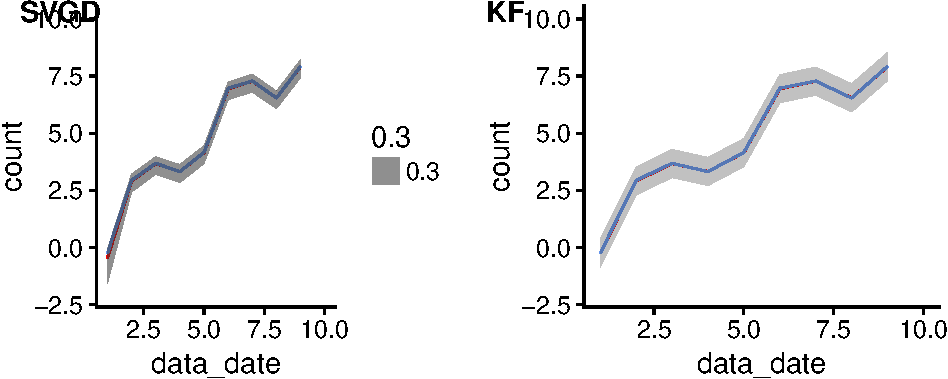
\includegraphics{ssvgd_files/figure-latex/unnamed-chunk-2-1.pdf}

\subsection{Poisson Observation Model With Seasonal State-Space
Dynamics}\label{poisson-observation-model-with-seasonal-state-space-dynamics}

In order to evaluate the performance on more involved dynamics we
consider the following state-space model.
\[\begin{pmatrix} X_{t,1} \\ X_{t,2} \end{pmatrix} = \begin{pmatrix} cos(2\pi/s) & sin(2\pi/s) \\ -sin(2\pi/s) & cos(2\pi/s) \end{pmatrix} \begin{pmatrix} X_{t-1,1} \\ X_{t-1,2} \end{pmatrix} \]
\[Y_t \sim Pois(e^{X_{t,1}})\]

\begin{verbatim}
## Loading required package: rbiips
\end{verbatim}

\begin{verbatim}
## Loading required package: coda
\end{verbatim}

\begin{verbatim}
## Loading required package: MASS
\end{verbatim}

\begin{verbatim}
## 
## Attaching package: 'MASS'
\end{verbatim}

\begin{verbatim}
## The following object is masked from 'package:dplyr':
## 
##     select
\end{verbatim}

\begin{verbatim}
## ##
## ## Markov Chain Monte Carlo Package (MCMCpack)
\end{verbatim}

\begin{verbatim}
## ## Copyright (C) 2003-2018 Andrew D. Martin, Kevin M. Quinn, and Jong Hee Park
\end{verbatim}

\begin{verbatim}
## ##
## ## Support provided by the U.S. National Science Foundation
\end{verbatim}

\begin{verbatim}
## ## (Grants SES-0350646 and SES-0350613)
## ##
\end{verbatim}

\begin{verbatim}
## * Parsing model in: /home/gcgibson/ssvgd/bug_files/seasonal_pois.bug
\end{verbatim}

\begin{verbatim}
## Warning in biips_model(seasonal_model_file, data = seasonal_data,
## sample_data = FALSE): Unused variables in data: G, mean_sigma_init,
## cov_sigma_init, mean_x_init
\end{verbatim}

\begin{verbatim}
## * Compiling model graph
##   Declaring variables
##   Resolving undeclared variables
##   Allocating nodes
##   Graph size: 121
\end{verbatim}

\begin{verbatim}
## * Assigning node samplers
## * Running SMC forward sampler with 100000 particles
##   |--------------------------------------------------| 100%
##   |**************************************************| 11 iterations in 9.29 s
\end{verbatim}

\begin{verbatim}
## [1] "python /home/gcgibson/ssvgd/python/seasonal.py  17, 18, 10, 16, 19, 11, 14, 20, 12, 13"
\end{verbatim}

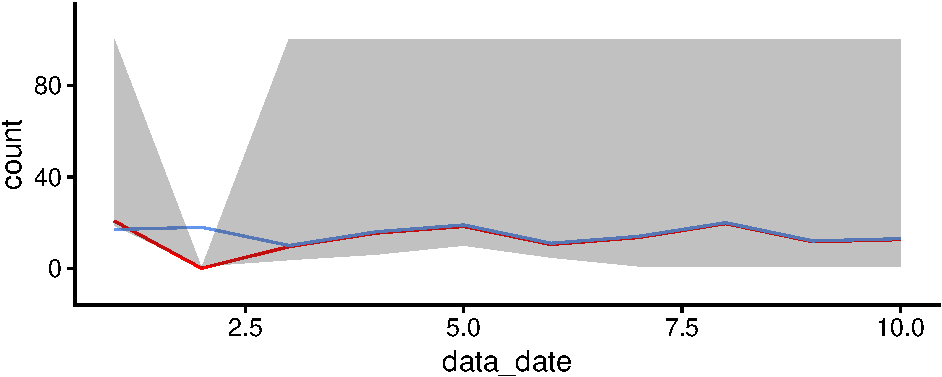
\includegraphics{ssvgd_files/figure-latex/unnamed-chunk-3-1.pdf}

\subsection{Divergent Particle Filter}\label{divergent-particle-filter}

We next investigate the ability of SSVGD to perform in the presence of
poor initialization. This is a well known issue with current particle
filter implementations: starting far from a plausible value of \(x_0\)
forces all particles to receive weight \(0\) under the likelihood,
leading to a degenerate filtering distribution. However, under SSVGD, we
can simply increase the number of iterations, allowing for arbitrarily
poor starting points. Standard particle filtering algorithms use
effective sample size as a measure of degeneracy. This is commonly
defined as \[S^{pf}_{eff} = \frac{1}{\sum_i (w_t^i)^2}\]. The common
rule of thumb is to not allow this quantity to drop below 50. The
natural translation of this metric into particle filtering is compute
the same metric based on the samples obtained by SSVGD.

\begin{verbatim}
## * Parsing model in: /home/gcgibson/ssvgd/bug_files/locally_level_1.bug
## * Compiling model graph
##   Declaring variables
##   Resolving undeclared variables
##   Allocating nodes
##   Graph size: 14
\end{verbatim}

\begin{verbatim}
## * Assigning node samplers
## * Running SMC forward sampler with 100 particles
##   |--------------------------------------------------| 100%
##   |**************************************************| 5 iterations in 0.00 s
\end{verbatim}

\begin{verbatim}
## * Diagnosis of variable: x[1:5] 
##   Filtering: POOR
##     The minimum effective sample size is too low: 8.152 
##     Estimates may be poor for some variables.
##     You should increase the number of particles
## .  Smoothing: POOR
##     The minimum effective sample size is too low: 4.629 
##     Estimates may be poor for some variables.
##     You should increase the number of particles
## .
\end{verbatim}

\begin{verbatim}
## [1] -0.4692  1.0525  0.7421  1.3743  1.5461
\end{verbatim}

\begin{verbatim}
## [1] "python /home/gcgibson/ssvgd/python/llg.py  1, 4, 0, 3, 2"
\end{verbatim}

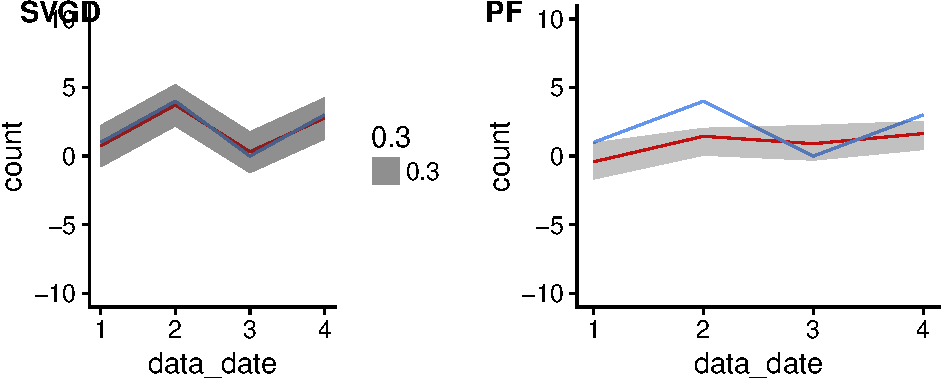
\includegraphics{ssvgd_files/figure-latex/unnamed-chunk-4-1.pdf}

\begin{verbatim}
## NULL
\end{verbatim}

\subsubsection{Diagnostics}\label{diagnostics}

Standard particle filtering algorithms use effective sample size as a
measure of degeneracy. This is commonly defined as
\[S_{eff} = \frac{1}{\sum_i (w_i)^2}\]. The common rule of thumb is to
not allow this quantity to fall below 50. Indeed, software
implementations such as Biips throws an error if the number of effective
particles falls below 50. We compute the effective sample size in an
analogous way to the particle filter, where \(w_i\) is defined as in the
SIR particle filter.

\begin{Shaded}
\begin{Highlighting}[]
\KeywordTok{library}\NormalTok{(knitr)}

\NormalTok{ess_df <-}\StringTok{ }\KeywordTok{data.frame}\NormalTok{(}\KeywordTok{seq}\NormalTok{(}\DecValTok{1}\NormalTok{:}\DecValTok{5}\NormalTok{),effect_size,out_smc$x$f$ess)}
\KeywordTok{colnames}\NormalTok{(ess_df) <-}\StringTok{ }\KeywordTok{c}\NormalTok{(}\StringTok{"t"}\NormalTok{,}\StringTok{"SSVGD ESS"}\NormalTok{, }\StringTok{"PF ESS"}\NormalTok{)}
\KeywordTok{kable}\NormalTok{(ess_df,}\DataTypeTok{caption=}\StringTok{"Effective Sample size"}\NormalTok{)}
\end{Highlighting}
\end{Shaded}

\begin{longtable}[]{@{}rrr@{}}
\caption{Effective Sample size}\tabularnewline
\toprule
t & SSVGD ESS & PF ESS\tabularnewline
\midrule
\endfirsthead
\toprule
t & SSVGD ESS & PF ESS\tabularnewline
\midrule
\endhead
1 & 3.4573 & 100.000\tabularnewline
2 & 0.2284 & 8.152\tabularnewline
3 & 23.1824 & 86.440\tabularnewline
4 & 1.2917 & 76.115\tabularnewline
5 & 2.2782 & 62.245\tabularnewline
\bottomrule
\end{longtable}

\paragraph{Results}\label{results}

In order to assess the accuracy of SSVGD we consider multiple different
evaluation metrics. We evaluate the forecasts on both mean-square-error
and log-score. Log-scores were computed as follows,

\[p(y_{1:n}) = \int_{x_{1:n}} p(y_{1:n} | x_{1:n}) p(x_{1:n}) d_{x_{1:n}}\]

This can be approximated as

\[\frac{1}{k}\sum_{i=1}^k p(y_{1:n} | x^{(i)}_{1:n})\] That is, we take
a full trajectory \(x_{1:n}\) and compute the log-probability of
\(y_{1:n}\). Note that this is equivalent to taking the average weight
at each step.

\begin{Shaded}
\begin{Highlighting}[]
\NormalTok{log_p <-}\StringTok{ }\KeywordTok{c}\NormalTok{()}
\NormalTok{for (i in }\DecValTok{1}\NormalTok{:}\KeywordTok{nrow}\NormalTok{(weights))\{}
  \NormalTok{log_p <-}\StringTok{ }\KeywordTok{c}\NormalTok{(log_p,}\KeywordTok{mean}\NormalTok{(weights[i,]))}
\NormalTok{\}}



\NormalTok{ll_df <-}\StringTok{ }\KeywordTok{data.frame}\NormalTok{(}\KeywordTok{sum}\NormalTok{(log_p),out_smc$log_marg_like)}
\KeywordTok{colnames}\NormalTok{(ll_df) <-}\StringTok{ }\KeywordTok{c}\NormalTok{(}\StringTok{"SSVGD"}\NormalTok{,}\StringTok{"PF"}\NormalTok{)}
\KeywordTok{kable}\NormalTok{(ll_df,}\DataTypeTok{caption=}\StringTok{"Log Score"}\NormalTok{)}
\end{Highlighting}
\end{Shaded}

\begin{longtable}[]{@{}rr@{}}
\caption{Log Score}\tabularnewline
\toprule
SSVGD & PF\tabularnewline
\midrule
\endfirsthead
\toprule
SSVGD & PF\tabularnewline
\midrule
\endhead
-4.928 & -16.42\tabularnewline
\bottomrule
\end{longtable}

\subsection{Discussion}\label{discussion}

Sequential Stein Variational Gradient Descent offers a useful
alternative to traditional particle filtering. We are able to increase
the effective sample size using the same number of particles. We are
also able to approximate the true likelihood of the Kalman Filter with a
small number of particles. Further work is required to understand the
impact of the bandwith heuristic on the resulting predictive intervals.

\subsection{Bibliography}\label{bibliography}


\end{document}
